\documentclass[9pt, aspectratio=169]{beamer}
%\documentclass[9pt, aspectratio=169, handout]{beamer}

\usetheme{metropolis}
\setbeamertemplate{itemize items}{\faAngleRight}

\metroset{titleformat=smallcaps,block=fill,numbering=counter,progressbar=frametitle,sectionpage=none}
\setbeamersize{text margin left=5mm,text margin right=5mm} 
% \input{embed_video}
\usepackage{fontspec,minted}
\usepackage[scale=1]{ccicons}
\usepackage{metalogo}
\usepackage{xcolor,colortbl}
\usepackage{multicol,multirow,booktabs}
\usepackage{appendixnumberbeamer}
\usepackage{graphicx}
\usepackage{mismath}
\usepackage{bm}
\usepackage{fontawesome5}
\usepackage{csquotes}
%\usepackage[backend=biber, natbib, sorting=nyt, doi=true, url=false, url=false, isbn=false, maxbibnames=10]{biblatex}
%\addbibresource{../../utils/refs.bib}

\usepackage[spanish, es-nodecimaldot]{babel}
\deftranslation[to=spanish]{Definition}{Definición}
\deftranslation[to=spanish]{Theorem}{Teorema}
\deftranslation[to=spanish]{Example}{Ejemplo}

\usepackage{mathtools, mathrsfs}
\usefonttheme{professionalfonts}
\usepackage{textcomp, wasysym}

\setsansfont[BoldFont={Iwona Bold}, Numbers={Lining, Proportional}]{Iwona Light}
% \setmathsfont(Digits)[Numbers={Lining, Proportional}]{Fira Sans Light}
\setmonofont[Scale=MatchLowercase]{DejaVu Sans Mono}

\setbeamercolor{alerted text}{fg=red,bg=black!2}
\setbeamercolor{progress bar}{fg=red,bg=red!2}
\setbeamertemplate{itemize item}{\faCaretRight}
\setbeamertemplate{itemize subitem}{ \faAngleRight}
\setbeamertemplate{blocks}[shadow=false]
\setbeamercolor{block title}{bg=black!30,fg=red}
\setbeamercolor{block body}{bg=black!20,fg=black}
\setbeamertemplate{theorem begin}
{%
\begin{\inserttheoremblockenv}
{%
\inserttheoremheadfont
%{Teorema:}
\inserttheoremname
\ifx\inserttheoremaddition\@empty\else\ : \inserttheoremaddition\fi%
\inserttheorempunctuation
}%
}
\setbeamertemplate{theorem end}{\end{\inserttheoremblockenv}}
\makeatother


 
\usepackage{gensymb,amssymb}
\usepackage{upquote}
\usepackage{cancel}
\usepackage{algpseudocode}
\algrenewcommand\algorithmicrequire{\textbf{Requiere}}
\algrenewcommand\algorithmicensure{\textbf{Devuelve}}
\setbeamertemplate{blocks}[shadow=false]

\newcommand{\cx}{\column{0.5\textwidth}}
\newcommand{\cw}[1]{\column{#1\textwidth}}

\author{Manuel Carlevaro}
\date{}
\institute{
  \vspace{6em}
  \centering
  {\tiny
  Universidad de Navarra \enspace • \enspace 2024 
} }

%% Operadores
\DeclareMathOperator{\sen}{sen}
\DeclareMathOperator{\senc}{senc}
\DeclareMathOperator{\sign}{sign}
\newcommand{\T}[1]{\underline{\bm{#1}}}
\DeclareMathOperator{\Tr}{Tr}
\DeclareMathOperator{\rg}{rg}
\DeclareMathOperator{\cond}{cond}

\usepackage{hyperref}
\hypersetup{
    colorlinks,
    citecolor=blue,
    filecolor=black,
    linkcolor=blue,
    urlcolor=blue
}
\urlstyle{same}


\usepackage{tikz}
\usetikzlibrary{shapes,shadows,arrows,positioning,matrix,chains,backgrounds,fit}

\tikzset{
    %Define standard arrow tip
    >=stealth',
    %Define style for boxes
    obj/.style={
           rectangle,
           rounded corners,
           draw, very thick,
           text width=10em, fill=green!20,
           minimum height=2em,
           text centered, drop shadow},
    proc/.style={
	    rectangle, rounded corners,
	    draw,fill=red!50,very thick,
	    text width=8em,minimum height=2em,
	    text centered, drop shadow},
    % Define arrow style
    pil/.style={
           ->,
           thick,
           shorten <=2pt,
           shorten >=2pt,}
}

%\setbeamertemplate{bibliography item}{%
  %\ifboolexpr{ test {\ifentrytype{book}} or test {\ifentrytype{mvbook}}
    %or test {\ifentrytype{collection}} or test {\ifentrytype{mvcollection}}
    %or test {\ifentrytype{reference}} or test {\ifentrytype{mvreference}} }
    %{\setbeamertemplate{bibliography item}{\faBook}}
    %{\ifentrytype{online}
            %{\setbeamertemplate{bibliography item}{\faGlobe}}
   %{\setbeamertemplate{bibliography item}{\faFileText}}}%
  %\usebeamertemplate{bibliography item}}

%\defbibenvironment{bibliography}
  %{\list{}
     %{\settowidth{\labelwidth}{\usebeamertemplate{bibliography item}}%
      %\setlength{\leftmargin}{\labelwidth}%
      %\setlength{\labelsep}{\biblabelsep}%
      %\addtolength{\leftmargin}{\labelsep}%
      %\setlength{\itemsep}{\bibitemsep}%
      %\setlength{\parsep}{\bibparsep}}}
  %{\endlist}
  %{\item}
%\newcommand{\bcite}[1]{\citeauthor{#1}, \citetitle{#1} (\citeyear{#1})}


\title{Introducción a la física}
\subtitle{Trabajo y energía}


\begin{document}
\maketitle
\begin{frame}
  \frametitle{Objetivos}
\Large

\begin{itemize}
 \item Aprender el concepto de trabajo realizado por una fuerza.
 \item Calcular el trabajo en casos simples.
 \item Aprender el teorema del trabajo y la energía cinética.
 \item Resolver problemas con fuerzas variables.
\end{itemize}
\end{frame}

\begin{frame}{Trabajo realizado por una fuerza}
\begin{columns} 
\cw{0.6}
\[ W = F \, s \]
\begin{itemize}
\item Se dice que la fuerza $\vec{F}$ \textbf{realizó un trabajo sobre} el objeto.
\item La unidad de trabajo en el S.I. es el Joule o Julio (\unit{J}).
\item $\qty{1}{J} = \qty{1}{N m} = \qty{1}{kg \cdot m^2 / s^2} $.
\item El concepto de \textbf{trabajo} en física no debe confundirse con el uso coloquial.
\end{itemize}
\cw{0.4}
\begin{center}
    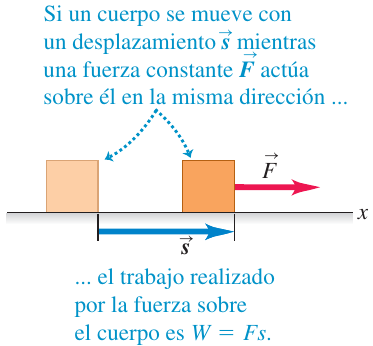
\includegraphics[width=0.8\textwidth]{figs/fig-01.png}
\end{center}
\end{columns}
\end{frame}

\begin{frame}{Fuerza no alineada con el desplazamiento}
    \begin{center}
        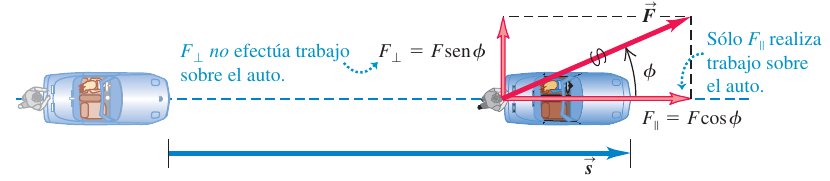
\includegraphics[width=0.7\textwidth]{figs/fig-02.png}
    \end{center}

\begin{multicols}{2}
    \begin{itemize}
        \item Si hay más de una fuerza aplicada, el desplazamiento puede no ser en la misma dirección que la fuerza cuyo trabajo nos interesa. En ese caso:
            \[ W = \vec{F} \cdot \vec{s} \]

        \item Se dice que la componente de una fuerza que es perpendicular al desplazamiento no realiza trabajo.
        \item El trabajo puede ser negativo.
        \item Para calcular el trabajo total de todas las fuerzas, 
            se calcula la fuerza neta (o resultante) $\vec{R}$ y se obtiene $W_{\text{total}} = \vec{R} \cdot \vec{s}$.
        \item Lo anterior es equivalente a obtener el trabajo de cada fuerza y sumar los trabajos al final.
        \item El trabajo es una magnitud \alert{escalar}.
    \end{itemize}
\end{multicols}
\end{frame}

\begin{frame}{Ejemplo}
\begin{columns}
\cx 
Una persona ejerce una fuerza constante de \qty{210}{N} sobre el coche averiado de la figura anterior, mientras lo empuja una distancia de \qty{18}{m}. Además, por tener un neumático desinflado, el empuje debe hacerse con un ángulo de \ang{30} para que avance de frente. a) ¿Cuánto trabajo hace la persona? b) Con ánimo de ayudar, esta persona empuja un segundo coche averiado con una fuerza constante $\vec{F} = \qty{160}{N} \hat{\bm{i}} - (\qty{40}{N}) \hat{\bm{j}}$. El desplazamiento resultante es $\vec{s} = (\qty{14}{m}) \hat{\bm{i}} + (\qty{11}{m}) \hat{\bm{j}}$. ¿Cuánto trabajo efectúa en este caso?
\pause

\cx
a) 
\begin{align*}
W &= F \, s\, \cos \phi \\
  &= (\qty{210}{N})(\qty{18}{m}) \cos \ang{30} = \qty{3.3e3}{J}
\end{align*}
\pause
b) 
\begin{align*}
    W &= \vec{F} \cdot \vec{S} = F_x \, x + F_y \, y \\
      &= (\qty{160}{N})(\qty{14}{m}) + (\qty{-40}{N})(\qty{11}{m}) \\
      &= \qty{1.8e3}{J}
\end{align*}
\end{columns}
\end{frame}

\begin{frame}{Trabajo positivo, negativo o cero}
    \begin{center}
        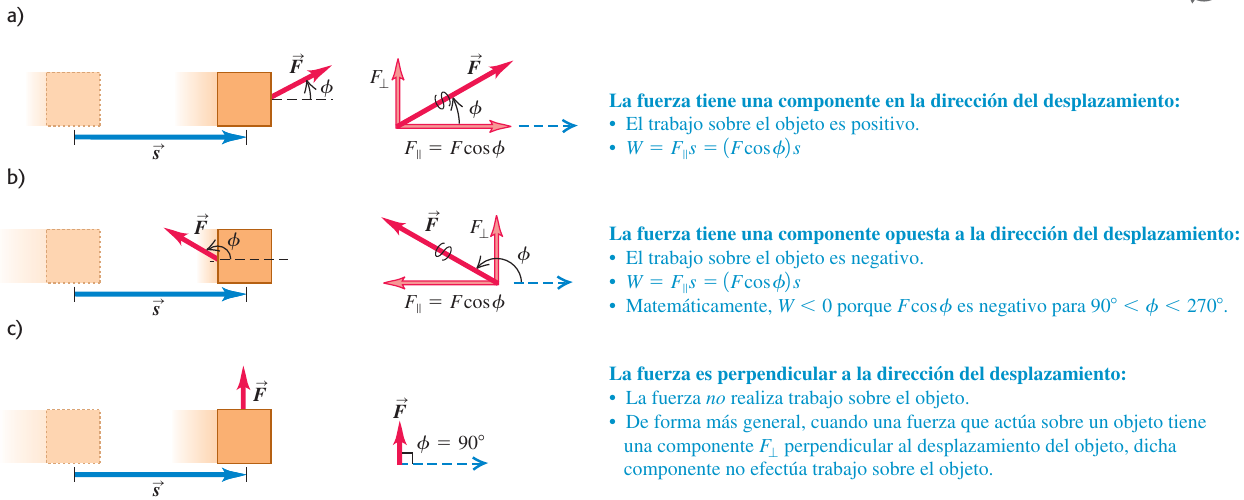
\includegraphics[width=1.0\textwidth]{figs/fig-03.png}
    \end{center}
\end{frame}

\begin{frame}{Energía cinética y el teorema trabajo-energía}
\begin{columns}
\cx
\begin{center}
    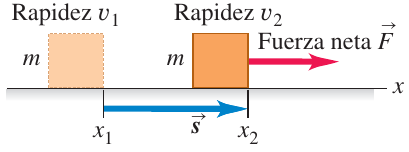
\includegraphics[width=0.7\textwidth]{figs/fig-04.png}
\end{center}
\begin{itemize}
    \item Cinemática:
        \begin{align*}
            v_2^2 &= v_1^2 + 2 a_x \, s \\
            a_x &= \frac{v_2^2 - v_1^2}{2 s}
        \end{align*}
    \item Segunda Ley de Newton:
        \begin{align*}
        F &= m \, a_x = m \frac{v_2^2 - v_1^2}{2s} \\
        F \, s &= \frac{1}{2} m v_2^2 - \frac{1}{2} m v_1^2 
        \end{align*}
    \end{itemize}
\pause
\cx
\begin{definition}[Energía cinética]
    \[ K = \frac{1}{2} m v^2 \]
\end{definition}
    \begin{itemize}
        \item La energía cinética es una magnitud \alert{escalar}.
        \item Depende solo de la masa y la rapidez de la partícula, no de su dirección.
        \item Nunca es negativa y solo puede ser cero si está en reposo
    \end{itemize}
\pause 

\begin{theorem}[Trabajo-energía]
El trabajo efectuado por la fuerza neta sobre una partícula es igual al cambio de energía cinética de la partícula:
\[ W_{\text{total}} = K_2 - K_1 = \Delta K \]
\end{theorem}
\end{columns}
\end{frame}

\begin{frame}{Ejemplo}
\begin{columns}
\cx
En un martinete, un martillo de acero con masa \qty{200}{kg} se levanta \qty{3.00}{m} sobre el tope de una viga vertical, que se está clavando en el suelo. El martillo se suelta, metiendo la viga otros \qty{7.4}{cm} en el suelo. Los rieles verticales que guían el martillo ejercen una fuerza de fricción constante de \qty{60}{N} sobre éste. Determine usando el teorema trabajo-energía a) la rapidez del martillo justo antes de golpear la viga, y b) la fuerza media que el martillo ejerce sobre la viga. 
\cx
\begin{center}
    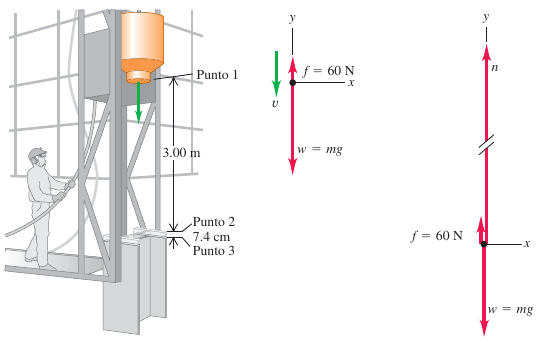
\includegraphics[width=1.0\textwidth]{figs/fig-05.png}
\end{center}
\end{columns}
\end{frame}

\begin{frame}{Fuerzas variables}
\begin{columns}
\cw{0.4}
\begin{center}
    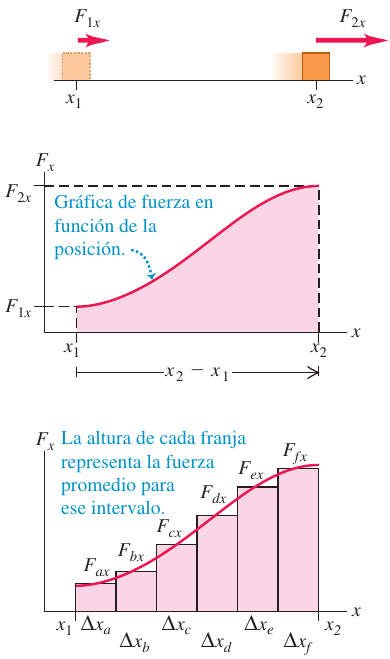
\includegraphics[height=0.8\textheight]{figs/fig-06.png}
\end{center}
\cw{0.6}
Aproximadamente:
\[ W = F_{ax} \Delta x_a + F_{bx} \Delta x_b + \cdots \]

En el límite donde el número de segmentos se hace muy grande y sus longitudes se hacen muy pequeñas:
\[ W = \int_{x_a}^{x_b} F_x \, dx \]

Se puede demostrar que el teorema trabajo-energía sigue siendo valido:
\[ W_{\text{total}} = K_2 - K_1 \]
\end{columns}
\end{frame}

\begin{frame}{Ejemplo: trabajo para comprimir o estirar un resorte}
\begin{columns}
    \cw{0.45}
    \begin{center}
        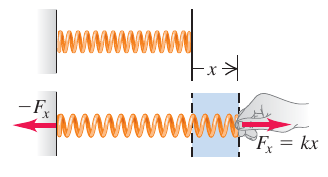
\includegraphics[width=0.7\textwidth]{figs/fig-07.png} \\
        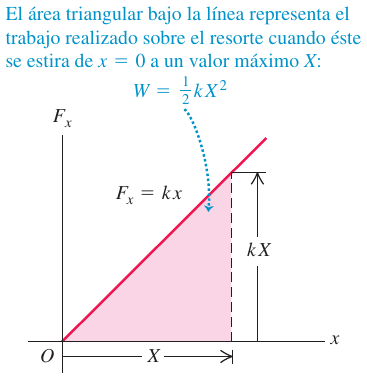
\includegraphics[width=0.7\textwidth]{figs/fig-08.png} 
    \end{center}
    \cw{0.55}
    Fuerza para estirar un resorte:
    \[ F_x = k \, x \]
    donde $k$ es la constante elástica del resorte (en \unit{N/m}).

    \[ W = \int_0^X F_x \, dx = \int_0^X kx \, dx = \frac{1}{2} k X^2 \]
    Si estiramos desde $x_1$ hasta $x_2$:
    \[ W = \int_{x_1}^{x_2} F_x \, dx = \int_{x_1}^{x_2} kx \, dx = \frac{1}{2} k x_2^2 - \frac{1}{2} k x_1^2 \]
\end{columns}
\end{frame}

\begin{frame}{Consideraciones importantes}
    \begin{columns}
        \cx
        \begin{center}
            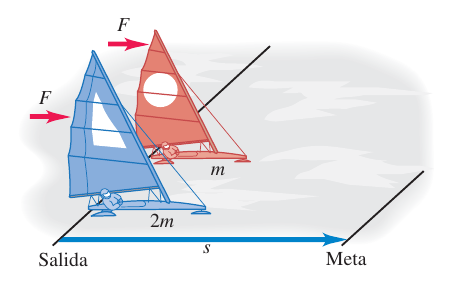
\includegraphics[width=1.0\textwidth]{figs/fig-09.png}
        \end{center}
        \cx
        \begin{itemize}
            \item ¿Cuál velero cruza la meta con mayor energía cinética?
            \item ¿Cuál llega primero?
        \end{itemize}
    \end{columns}
\end{frame}

\begin{frame}{Potencia}
\begin{columns}
    \cw{0.4}
\begin{definition}[Potencia media]
    \[ P_{\text{media}} = \frac{\Delta W}{\Delta t} \]
\end{definition}
\pause 
\bigskip

\begin{definition}[Potencia instantánea]
    \[ P = \lim_{\Delta t \rightarrow 0} \frac{\Delta W}{\Delta t} = \frac{dW}{dt} \]
\end{definition}
\pause
    \cw{0.6}
\begin{itemize}
    \item La unidad de potencia en el S.I. es el watt o vatio (\unit{W}).
    \item $\qty{1}{W} = \qty{1}{J/s} = \qty{1}{N \cdot m / s} = \qty{1}{kg \cdot m^2 / s^3} $
    \item Se puede hacer el mismo trabajo pero a diferente potencia.
    \item Se puede relacionar potencia con fuerza y velocidad. Si $\vec{F}$ es constante:
        \[ P = \frac{dW}{dt} = \frac{d}{dt}(\vec{F} \cdot \vec{x}) = \vec{F} \cdot \frac{d \vec{x}}{dt} = \vec{F} \cdot \vec{v} \]
        (Fórmula válida para cualquier situación en general.)
\end{itemize}
\end{columns}
\pause

\textbf{Otras unidades de potencia y energía:}
\begin{itemize}
    \item \textbf{Potencia:} $\qty{1}{hp} = \qty{746}{W}$ (caballo de potencia, \textit{horse power}).
    \item \textbf{Energía:} $\qty{1}{kW \cdot h} = \qty{1000}{J \cdot h / s} = \qty{3600000}{J} = \qty{3.6e6}{J}$
\end{itemize}
\end{frame}

\begin{frame}{Ejemplos}
    \begin{columns}[t]
\cx
\textbf{1.} El motor de un coche aplica una fuerza para moverlo y vencer el rozamiento con el asfalto y el aire que se le oponen. A \qty{50}{km/h} de rapidez la fuerza que se le opone es de \qty{1000.0}{N}, pero a \qty{100.0}{km/h} la fuerza que se le opone es más que el doble (\qty{3000.0}{N}). ¿Qué potencia desarrolla el motor en cada caso?

Si supongo que la fuerza que se opone es constante  de \qty{1000.0}{N} y la masa del coche \qty{800.0}{kg}, ¿qué potencia máxima debe desarrollar el motor para acelerar de \num{0.0} a \qty{100.0}{km/h} en \qty{10}{s}?

\cx
\textbf{2.} ¿Cuánta energía (en \unit{J} y en \unit{kWh}) consume una lámpara de \qty{100}{W} en una hora? ¿Qué potencia tiene en \unit{hp}?

\textbf{3.} El viento empuja las palas de un generador eólico de \qty{15.0}{m} de radio con \qty{40000}{N} de fuerza y hace que den una vuelta en \qty{10.0}{s}. El generador convierte la energía mecánica en eléctrica y mantiene encendido un sistema de iluminación de lámparas de \qty{100.0}{W}. ¿Cuántas lámparas están conectadas? ¿Qué sucede con el generador si súbitamente se apagan la mitad de las lámparas?

\end{columns}
\end{frame}



\end{document}
